% This is samplepaper.tex, a sample chapter demonstrating the
% LLNCS macro package for Springer Computer Science proceedings;
% Version 2.20 of 2017/10/04
%
\documentclass[runningheads]{llncs}
%
\usepackage{graphicx}
\usepackage{amsmath}
\usepackage{amssymb}
\usepackage{bm}
\usepackage{amsfonts}
\usepackage{subfig}
\graphicspath{{./imgs/}}

\begin{document}
%
\title{Normalizing Flows}
%
%\titlerunning{Abbreviated paper title}
% If the paper title is too long for the running head, you can set
% an abbreviated paper title here
%
\author{Abdul Fatir Ansari\inst{1} \and
Devamanyu Hazarika\inst{1} \and
Remmy A. M. Zen\inst{1}}
%
\authorrunning{CS6202 Project Report}
% First names are abbreviated in the running head.
% If there are more than two authors, 'et al.' is used.
%
\institute{National University of Singapore \\
\email{\{abdulfatir,devamanyu,remmy\}@u.nus.edu}}
%
\maketitle              % typeset the header of the contribution
%
\begin{abstract}


\keywords{Normalizing flows \and .}
\end{abstract}
%
%
%
\section{Introduction}
\section{Background}
\subsection{Autoencoder}
\subsection{Variational Autoencoder}


\section{Normalizing Flows}

Before defining normalizing flows, let's consider a univariate distribution with density function $p(x)$. Define a continuous, differentiable, and increasing function $f$. Define $y = f(x)$ where $x \sim p(x)$. The density function of the random variable $Y$ can then be derived analytically using the Cumulative Distribution Function (CDF) as follows.

\begin{align}
F_{Y}(y) &= P(Y \leq y)\\
&= P(f(X) \leq y)\\
&= P(X \leq f^{-1}(y)) = F_{X}( f^{-1}(y))
\end{align}

We end up with the CDF of the random variable $X$ at the point $f^{-1}(y)$. Now, $p(y) = F_{Y}'(y)$ by definition, where

\begin{align}
F_{Y}(y) = F_{X}( f^{-1}(y)) = \int_{-\infty}^{ f^{-1}(y)}p(x) dx
\label{eq:cdfy}
\end{align}

Differentiating Eq. (\ref{eq:cdfy}) with respect to $y$ (using the Fundamental Theorem of Calculus and the chain rule) we get

\begin{align}
p(y) = p(f^{-1}(y))\cdot \frac{df^{-1}}{dy}
\label{eq:incfn}
\end{align}

When $f$ is a decreasing function, we get $p(y) = p(f^{-1}(y))\cdot \frac{df^{-1}}{dy}$.  For an invertible function in general, Eq. (\ref{eq:incfn}) can be written as 

\begin{align}
p(y) = p(f^{-1}(y))\cdot \left|\frac{df^{-1}}{dy}\right|
\label{eq:covuv}
\end{align}

Eq. (\ref{eq:covuv}) can be extended to the multivariate case where the derivative is replaced by the determinant of the Jacobian matrix $J$

\begin{align}
p(\mathbf{y}) = p(f^{-1}(\mathbf{y}))\cdot \left|\det\frac{\partial f^{-1}}{\partial\mathbf{y}}\right| = p(f^{-1}(\mathbf{y}))\cdot \left|\det\frac{\partial f}{\partial f^{-1}(\mathbf{y})}\right|^{-1}
\label{eq:covmv}
\end{align}

In the above equation, the second equality comes from the inverse function theorem. Successive applications of such smooth, invertible transformation on a random variable with known density is called a \textit{normalizing flow}.

 Computation of the probability density of the transformed random variable requires the computation of the determinant of the Jacobian matrix which is computationally expensive as it scales with $O(d^3)$ where $d$ is the dimensionality of the random variable. Developing transformations with cheap determinant computation has been the primary focus of many recent works.
\section{Applications}
Literature on normalizing flows can be broadly classified into two parts: ones using normalizing flows for improved variational inference and ones using normalizing flows for density estimation.
\subsection{Variational Inference}
Variational methods perform inference by approximating the true posterior $p(z|x)$ using a simpler variational family $q_{\phi}(z|x)$. Recent works have focused on improving the variational posterior used in the VAE which is generally set to a multivariate normal distribution with diagonal covariance matrix $\mathcal{N}(\bm{\mu}, \sigma^2\mathbf{I})$. It is clear that such a simplistic, unimodal choice for the posterior can be arbitrarily far away from the true posterior which can be a complex multi-modal distribution. 

Recent works seek to convert samples from a simple variational posterior (such as the multivariate normal distribution) into a richer distribution by applying a series of smooth, invertible transformations or a flow. Let $\mathbf{z}_0$ be a sample from a simple distribution $q_0(\mathbf{z}_0)$ and $\mathbf{z}_K$ be a sample obtained by applying a flow of length $K$ on $\mathbf{z}_0$, i.e., $\mathbf{z}_K = f_K \circ f_{K-1} \circ \dots \circ f_1 (\mathbf{z}_0)$. Using Eq. (\ref{eq:covmv}), the density function $q_K(\mathbf{z}_K)$ is given by

\begin{align}
q_K(\mathbf{z}_K) = q_0(\mathbf{z}_0)\prod_{k=1}^K\left|\det \frac{\partial f_k}{\partial \mathbf{z}_{k-1}}\right|^{-1}\label{eq:qzk}
\end{align}

The variational lower bound (or evidence lower bound) in VAEs (Eq. ()) can now be modified by setting $q(\mathbf{z}|\mathbf{x}) = q_K(\mathbf{z}_K|\mathbf{x})$
\begin{align}
\mathcal{L} &= \mathbb{E}_{q(\mathbf{z}_K|\mathbf{x})}\left[\log p_\theta(\mathbf{x}, \mathbf{z}_K) - \log q(\mathbf{z}_K|\mathbf{x})\right]\\
&= \mathbb{E}_{q(\mathbf{z}_0|\mathbf{x})}\left[\log p_\theta(\mathbf{x}, \mathbf{z}_K) - \log q(\mathbf{z}_K|\mathbf{x})\right]\label{eq:lotus}
\end{align}
where $q(\mathbf{z}_0|\mathbf{x})$ is the simple initial density. Plugging in Eq. (\ref{eq:qzk}) into Eq. (\ref{eq:lotus}), we get a modified bound for flow-based VAEs
\begin{align}
\mathcal{L} &= \mathbb{E}_{q_0(\mathbf{z_0}|\mathbf{x})}\left[\log p(\mathbf{x},\mathbf{z}_K) - \log q_0(\mathbf{z}_0|\mathbf{x}) + \sum_{k=1}^K\log\left|\det \frac{\partial f_k}{\partial \mathbf{z}_{k-1}}\right| \right]
\end{align}
\subsubsection{Planar and Radial Flows} 
Planar and Radial Flows \cite{rezende2015variational} are one of the earliest flows proposed in the context of variational inference. 

Planar flows use functions of the form
\begin{align}
f(\mathbf{z}) = \mathbf{z} + \mathbf{u}h(\mathbf{w}^\top\mathbf{z} + b)
\label{eq:planarfn}
\end{align}

where $\mathbf{u},\mathbf{w}\in \mathbb{R}^d$, $b \in \mathbb{R}$, and $h$ is an element-wise non-linearity such as $\tanh$.

The Jacobian is then given by
\begin{align}
\det\frac{\partial f(\mathbf{z})}{\partial \mathbf{z}} =(1 + h'(\mathbf{w}^\top\mathbf{z} + b)\mathbf{w}^\top\mathbf{u})
\end{align}
which can be computed in $O(d)$ time.

Radial flows use functions of the form
\begin{align}
f(\mathbf{z}) = \mathbf{z} + \beta h(\alpha,r)(\mathbf{z}-\mathbf{z}_0)
\label{eq:radialfn}
\end{align}

where $\alpha \in \mathbb{R}^+$, $\beta \in \mathbb{R}$, $h(\alpha,r) = (\alpha + r)^{-1}$ and $r = \vert\vert\mathbf{z} - \mathbf{z}_0\vert\vert$.

The Jacobian is then given by
\begin{align}
\det\frac{\partial f(\mathbf{z})}{\partial \mathbf{z}} = \left(1 + \beta h(\alpha,r) + \beta h'(\alpha,r)r\right)(1+\beta h(\alpha,r))^{d-1}
\end{align}
For a detailed derivation of Jacobians of Planar and Radial flows please refer Appendix. Fig. \ref{fig:planarradial} shows how planar and radial flows change a standard normal distribution.

\begin{figure}
	\centering
	\subfloat[Initial Density]{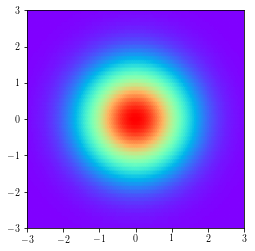
\includegraphics[width=0.24\textwidth]{planar-q0}}
	\subfloat[Planar Flow]{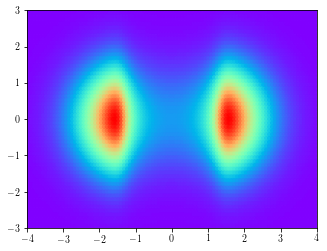
\includegraphics[width=0.31\textwidth]{planar-q1}}
	\subfloat[Radial Flow]{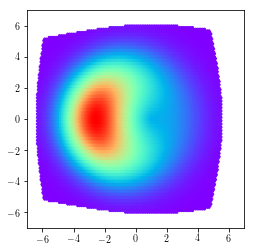
\includegraphics[width=0.24\textwidth]{radial-q1}}
	\caption{Change in standard normal density on application of length 1 planar and radial flows.}
	\label{fig:planarradial}
\end{figure}

\subsubsection{Inverse Autoregressive Flows}
~\cite{kingma2016improved}


\subsection{Density Estimation}

\subsubsection{Non-linear Independent Components Estimation}
\subsubsection{Real-valued Non-Volume Preserving}

\section{Normalizing Flows in Probabilistic Programming Languages}
~\cite{dillon2017tensorflow}

\section{Recent Advances}
\subsection{Pixel Recurrent Neural Network}
~\cite{oord2016pixel}
\subsection{Wavenet}
~\cite{van2016wavenet}
\subsection{Glow}
~\cite{kingma2018glow}



\section{Conclusion}


\section{Contribution}

%
% ---- Bibliography ----
%
% BibTeX users should specify bibliography style 'splncs04'.
% References will then be sorted and formatted in the correct style.
%
% \bibliographystyle{splncs04}
% \bibliography{mybibliography}
%
\bibliographystyle{splncs04}
\bibliography{ref} 

\appendix

\section{Appendix (Abdul Fatir Ansari)}


The Jacobian is then given by

\begin{align*}
\frac{\partial f(\mathbf{z})}{\partial \mathbf{z}} = \mathbf{I} + \mathbf{u}h'(\mathbf{w}^\top\mathbf{z} + b)\mathbf{w}^\top
\end{align*}

Now, using the matrix determinant lemma

\begin{align}
\det\frac{\partial f(\mathbf{z})}{\partial \mathbf{z}} &= (1 + h'(\mathbf{w}^\top\mathbf{z} + b)\mathbf{w}^\top\mathbf{I}^{-1}\mathbf{u})\det(\mathbf{I})\\
&=(1 + h'(\mathbf{w}^\top\mathbf{z} + b)\mathbf{w}^\top\mathbf{u})\label{eq:planar-det}
\end{align}

\section{Appendix (Devamanyu Hazarika)}
\section{Appendix (Remmy Zen)}

\end{document}
